\documentclass[12pt]{article}       % 設定文件類型為 article,字體大小為 12pt
\usepackage[T1]{fontenc}            % 設定 T1 字型編碼,確保特殊字元的正確顯示
\usepackage{lmodern}                % 強制使用 Latin Modern 字型,提高可讀性和相容性
\usepackage{fontspec}               % 允許使用 OpenType 和 TrueType 字型
\usepackage{graphicx}               % 支援插入圖片
\usepackage{amsmath}                % 提供數學環境和公式支持
\usepackage{csquotes}               % 提供引用格式支援
\usepackage{comment}                % 提供多行註解
\usepackage{ragged2e}
\usepackage{amsmath}
\usepackage{float}

%biber NSTC_project

%=================================================={{{參考文獻設定}}}==================================================

\usepackage[style=ieee, maxnames=99]{biblatex}          % 設定參考文獻格式為 IEEE,最多顯示 99 個作者
\addbibresource{NSTC_project.bib}                       % 添加參考文獻檔案 references.bib
\renewcommand{\bibfont}{\fontspec{Times New Roman}}     % 設定參考文獻字體為 Times New Roman
\renewcommand{\UrlFont}{\fontspec{Times New Roman}}     % 設定 URL 連結字體為 Times New Roman
\DeclareFieldFormat{url}{\url{#1}}                      % 格式化 URL
\bibliography{your_bib_file}                            % 引用你的 .bib 文件

%=================================================={{{目錄設定}}}==================================================

\usepackage{tocloft} % 自訂目錄格式

% 設定目錄的點線填充樣式
\renewcommand{\cftsecleader}{\cftdotfill{\cftdotsep}}           % 章節(section)
\renewcommand{\cftsubsecleader}{\cftdotfill{\cftdotsep}}        % 小節(subsection)
\renewcommand{\cftsubsubsecleader}{\cftdotfill{\cftdotsep}}     % 子小節(subsubsection)

% 設定圖目錄與表目錄的點線
\renewcommand{\cftdotsep}{1}  % 設定點的間距,使其在所有目錄(含圖、表)中都有效

% 設定目錄標題格式,使目錄、圖目錄、表目錄標題一致
\renewcommand{\contentsname}{\centering \LARGE \textbf{目錄}}    % 目錄標題置中,加粗
\renewcommand{\listfigurename}{\centering \LARGE \textbf{圖目錄}} % 圖目錄標題置中,加粗
\renewcommand{\listtablename}{\centering \LARGE \textbf{表目錄}} % 表目錄標題置中,加粗


%=================================================={{{字體設定}}}==================================================

% 設定英文字體
\newfontface\englishfont{Times New Roman}               % 自訂英文字體命令 \englishfont,使用 Times New Roman

\setmainfont[
    ItalicFont={Times New Roman Italic},                % 設定斜體
    BoldFont={Times New Roman Bold},                    % 設定粗體
    BoldItalicFont={Times New Roman Bold Italic}        % 設定粗斜體
]{Times New Roman}                                      % 設定主要英文字體為 Times New Roman

% 設定中文字體

\usepackage{xeCJK}                                      % 使用 xeCJK 宏包以支援中文
\renewcommand{\figurename}{圖}                           % 設定圖表名稱
\renewcommand{\tablename}{表}                            % 修改表格標題為「表」
\setCJKmainfont[BoldFont={標楷體-繁}, ItalicFont={標楷體-繁}] {標楷體-繁}

%=================================================={{{版面設定}}}==================================================

% 設定頁面邊界,適用 A4 紙張
\usepackage[top=2cm, bottom=2cm, left=2cm, right=2cm, a4paper]{geometry}

% 設定行距與段落格式
\usepackage{setspace}
\onehalfspacing % 設定 1.5 倍行距
\setlength{\parskip}{6pt} % 設定段落間距 6pt
\setlength{\parindent}{2em} % 設定段落首行縮排 2 個字元

%=============================================================================================================================
%=============================================================================================================================
%=============================================================================================================================

\begin{document}

\pagenumbering{roman}  
\setcounter{page}{1}  % 從 I 開始

%=================================================={{{中文摘要}}}==================================================

\section*{\centering 摘要}  % 只讓標題置中
\addcontentsline{toc}{section}{摘要}  % 手動加入摘要到目錄

%==============================摘要內容==============================

\hspace{2em}
本研究計畫旨在開發一套智慧交通巡檢系統,利用四軸飛行載具(Unmanned Aerial Vehicle, UAV)進行違規停車車輛的偵測。
不同於以往先判斷紅線位置再確認車輛是否違規的方法,本研究透過四軸飛行器的GPS定位資訊來判斷車輛是否違規,避免車輛停在紅線上或完全遮掩紅線的情況。
由於系統僅檢視違規區域,此方法還能加快巡邏速度,提升巡邏效率。

本系計畫統採用YOLOv7物件偵測模型進行即時車輛辨識,結合飛行器的姿態與相機拍攝角度,
利用逆透視變換(Inverse Perspective Mapping,IPM)定位,將偵測結果轉換為地面上的絕對位置,這樣能夠快速確定違規停車車輛的位置。
透過事先建立的資料庫,無人機將比對飛越指定區域所拍攝的影像,並即時偵測違規車輛,記錄其位置。
該系統的優勢在於高效的監控能力,能夠大幅減少設備投資成本,並提升違規車輛檢測的靈活性和即時性。

\vspace{1.5em}
\noindent 關鍵字:即時物件偵測、四旋翼無人機、空間對位
%==============================摘要內容==============================
\newpage  % 插入換頁命令,將目錄和後續內容分開

%=================================================={{{英文摘要}}}==================================================
\section*{\centering Abstract}  % 只讓標題置中
\addcontentsline{toc}{section}{Abstract}  % 手動加入摘要到目錄
%==============================摘要內容==============================
\hspace{2em}This research aims to develop an intelligent traffic inspection system utilizing unmanned aerial vehicles (UAVs) to detect illegally parked vehicles.
Unlike conventional methods that first identify the location of red lines and then verify whether vehicles are violating parking regulations, this system determines whether a vehicle is in violation by using the UAV's GPS positioning information, preventing vehicles from parking on or completely covering red lines.
Since the system only inspects the violation areas, this approach helps speed up patrol operations and enhance overall patrol efficiency.

This research adopts the YOLOv7 object detection model for real-time vehicle identification, combined with the UAV's attitude and camera angle.
By using Inverse Perspective Mapping, the system locates and converts the detection results into absolute ground positions, allowing for quick identification of illegally parked vehicles.
Through a pre-established database, the UAV compares the images captured while flying over designated areas and immediately detects violation vehicles, recording their locations. The advantage of this system lies in its efficient monitoring capability, significantly reducing equipment investment costs and improving the flexibility and immediacy of illegal parking detection.

\vspace{1.5em}
\noindent Keyword: Real-time Object Detection, Quadcopter, Georeferencing
%==============================摘要內容==============================
\newpage  % 插入換頁命令,將目錄和後續內容分開

%=================================================={{{目錄}}}==================================================

\begin{center}
    \tableofcontents    % 生成目錄
    \newpage  % 插入換頁命令,將目錄和後續內容分開
    \addtocontents{toc}{\protect\setcounter{tocdepth}{0}} % 暫時關閉目錄深度,讓圖目錄不顯示在目錄中
    \listoffigures      % 生成圖目錄
    \addtocontents{toc}{\protect\setcounter{tocdepth}{2}} % 恢復目錄深度(如果你的章節結構需要更深層級,請調整數值)
    \newpage  % 插入換頁命令,將目錄和後續內容分開
    \listoftables       % 生成表目錄
\end{center}
    
    \newpage  % 插入換頁命令,將目錄和後續內容分開
%=================================================={{{內容開始}}}==================================================

\pagenumbering{arabic}  % 開始使用阿拉伯數字頁碼
\setcounter{page}{1}  % 設定頁碼從 1 開始

%\englishfont{this is an example of mixed English and Chinese.}

\section{\centering 緒論}

\subsection{研究背景} 
%==============================內文==============================
\hspace{2em}
無人機(Unmanned Aerial Vehicle, UAV)技術近年來快速發展,整合各種附加設備並隨著飛行控制與自動化技術的成熟,在軍事、執法及科技應用領域取得顯著成效。
四軸旋翼無人機因其安全性高、成本低的優勢,已廣泛應用於各種場景,其中攝影與錄影功能尤為重要。
無人機擁有比傳統攝影設備更廣的視角,且受環境限制較小,使其在大範圍場景捕捉方面表現優異,優於傳統監控方式。

在交通監控領域,無人機的靈活性和效率遠勝於傳統固定式監控設備,如固定式照相桿雖能執行監控任務,但監測範圍有限且設備成本較高。
隨著無人機技術的進步,其在交通巡檢方面展現出極大的應用潛力,特別是在違規停車偵測方面,無人機能夠提供更靈活且高效的解決方案。
目前,中國部分城市已開始運用無人機進行科技執法\cite{chinatimes2019},台北市與台中市警察局亦已成立無人機機隊\cite{cna_2022}\cite{tai_2021},用於交通監測與執法,並協助執法人員即時掌握交通狀況,提升執法效率。

\begin{figure}[H]
    \centering
    \renewcommand{\figurename}{圖} %顯示圖1,不是figureat1
    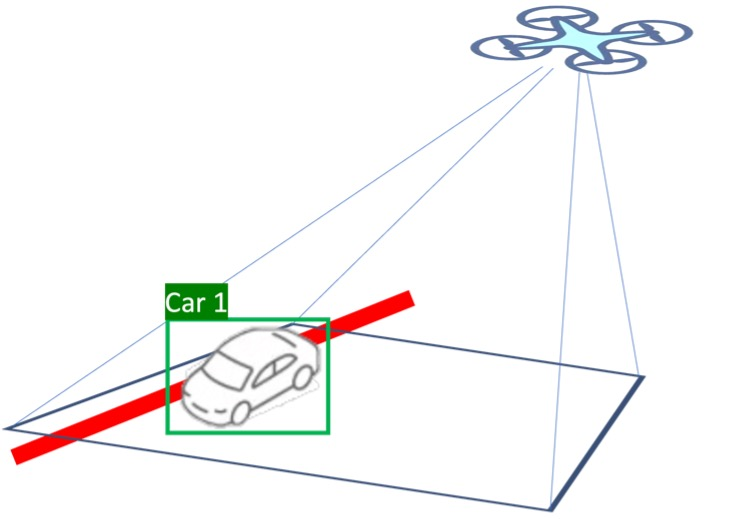
\includegraphics[width=0.7\textwidth]{research_problem1.jpg}     %圖片檔案名稱
    \caption{無人機偵測違停車輛示意圖}    %圖片檔案名稱
    \label{fig:research_problem1}    %為圖片添加標籤
    %圖\ref{fig:無人機偵測違停車輛示意圖}
\end{figure}
%==============================內文==============================

\subsection{研究動機} 
%==============================內文==============================
\hspace{2em}目前的研究和應用大多針對車輛橫跨紅線進行判斷,但對於完全蓋住紅線或停在紅線與白線交界處的情況,現有方法無法準確判斷車輛是否違停。
因此,本研究計畫的動機在於利用無人機的GPS位置資訊來判斷車輛的違規情形,避免車輛完全遮掩紅線或停在紅線邊界處的情況。
如圖\ref{fig:research_problem2} 所示。
並通過建立資料庫並使用無人機拍攝影像,比對車輛所處位置與違規區域,能夠快速偵測違規車輛並進行即時回報,進一步提升交通執法的效率與靈活性。

\begin{figure}[H]
    \centering
    \renewcommand{\figurename}{圖} %顯示圖1,不是figureat1
    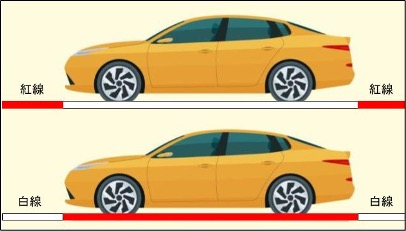
\includegraphics[width=0.7\textwidth]{research_problem2.jpg}     %圖片檔案名稱
    \caption{本計畫研究問題之示意圖}    %圖片檔案名稱
    \label{fig:research_problem2}    %為圖片添加標籤
    %圖\ref{fig:example1}
\end{figure}
%==============================內文==============================

\subsection{研究問題} 
%==============================內文==============================
\hspace{2em}利用無人機拍攝出的影像辨識出沿路車輛,利用無人機本身 GPS 位置,換算出影像中車輛之位置,比對車輛所在位置是否可以停車,
以判斷車輛否違規,若有違規情形,回傳車輛位置並將其建立成資料庫,以便於人員複查或是違規檢舉。研究問題可以分為三大項,違規車輛偵測、影像處理、空間對位。
%==============================內文==============================

\subsubsection{違規車輛偵測}
%==============================內文==============================
\hspace{2em}為了精確偵測違規停放的車輛,本系統採用先進的影像辨識技術,利用 YOLOv7 進行即時車輛偵測,確保能快速且準確地識別影像中的車輛。
透過無人機高空巡檢,可大範圍覆蓋監控區域。此外,系統將結合 GPS 位置資訊,以判斷車輛是否位於可能的違規區域,
如紅線停車區、消防通道或人行道上,進一步提高偵測的可靠性與準確性。
%==============================內文==============================

\subsubsection{影像處理}
%==============================內文==============================
\hspace{2em}本計畫將利用鏡頭往斜下的角度拍攝而非垂直向下。以斜下角度拍攝的特點是相較於垂直向下拍攝可以擁有較大的視野範圍。
而採用無人機的 GPS位置資訊判斷,無人機拍攝圖片中每個像素與實際地面之關係格外重要,除了無人機上相機的傾角,
還需整合無人機在飛行時的對地高度、翻滾角 (Roll)、俯仰角(Pitch)、偏航角(Yaw)等慣性測量單元(Inertial measurement unit, IMU),
並依據該照片拍攝時之IMU資訊做正射投影,運算每個像素與無人機之間的相對位置,並依照無人機的GPS位置準確定位違規車輛之位置。
%==============================內文==============================

\subsubsection{空間對位}
%==============================內文==============================
\hspace{2em}為確保偵測結果的精準性,系統將進行空間對位處理,以克服飛行器姿態變化、鏡頭視角與透視變形等因素所造成的誤差。
透過飛行器的 IMU(慣性測量單元)數據與 GPS 定位資訊,獲取無人機的姿態與拍攝角度,並利用透視變換技術將影像坐標轉換為地面絕對位置。
最後,系統將偵測出的車輛位置與電子地圖上的違規區域進行重合度分析,精確確認車輛是否確實違規停放,並輸出違規證據以供後續處理。
%==============================內文==============================

\section{\centering 文獻探討與回顧}

\subsection{應用YOLOv7於車輛物件偵測}
%==============================內文==============================
\hspace{2em}違規停車偵測的部分預計使用物件偵測深度神經網路,找出車輛位置,以判斷車輛是否違規,利用物件偵測深度神經網路,不管是在標註樣本或是進行訓練上都可以節省許多的時間,並且擁有較高的準確度。
本計畫採用知名的物件偵測深度神經網YOLO,其全名為You Only Look Once,首次出現於 2015 年,由 Joseph Redmon 和 Ali Farhadi 等人提出\cite{ren_2015}。
YOLO能夠在實時情況下執行物體檢測,這意味著它可以快速地識別圖像中的物體,並且適用於需要即時反饋的應用場景,相較於其他物體檢測算法,YOLO算法在準確性上表現出色,能夠有效地檢測各種大小和形狀的物體,相對於其他複雜的物體檢測算法而言,實現起來相對簡單,這使得它受到廣泛的歡迎並且易於應用於各種領域,有實時檢測、高準確性、簡單易用、可擴展性等優點。

\begin{figure}[H]
    \centering
    \renewcommand{\figurename}{圖} %顯示圖1,不是figureat1
    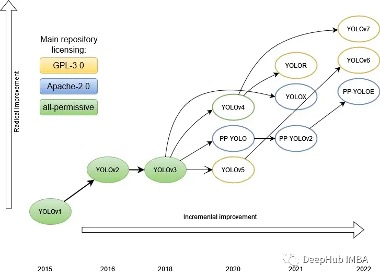
\includegraphics[width=0.7\textwidth]{yolov7_1.jpg}     %圖片檔案名稱
    \caption{YOLO各版本演進圖\cite{tencent2023}}    %圖片檔案名稱
    \label{fig:yolov7_1}    %為圖片添加標籤
    %如圖\ref{fig:yolov7_1}所示
\end{figure}

本研究選用YOLOv7\cite{wang2023yolov7}作為物件偵測算法,其為YOLO系列中的高效版本,具有優異的準確性與速度(如圖\ref{fig:yolov7_2} 所示)。YOLOv7屬於one stage物件偵測方法,能夠在單次運行中同時完成位置偵測與物件分類,相較於two stage方法,其運算速度更快,且準確度仍維持在可接受範圍內。
YOLOv7在架構設計上延續了YOLOv3的基本結構,包括主幹網路(Backbone)、連接層(Neck)與檢測頭(Head),並透過引入新技術進一步提升效能(如圖\ref{fig:yolov7_3} 所示)。
Backbone負責特徵提取,輸入圖像經過多層卷積運算,從B1至B5逐步提取更加豐富的特徵資訊,特徵圖尺寸逐漸縮小,但通道數量增加;Neck透過上採樣(upsampling)擴增特徵圖,並透過橫向連結融合不同層級的特徵,使模型能夠有效學習多尺度資訊;
Head則負責最終檢測結果的輸出,透過下採樣(subsampling)還原金字塔結構,最終產生多種解析度的特徵圖(P3、H4、H5)以適應不同大小的物件偵測需求。此外,YOLOv7透過模型重參數化(Re-parameterized model)改進模型結構以提高推理速度,並提出Extend-ELAN(E-ELAN),在不破壞梯度傳播的情況下增強網路學習能力。
透過這些技術,YOLOv7在物件偵測任務中展現了更優異的效能,能夠在高準確度與低延遲之間取得良好平衡,適用於多種應用場景。

\begin{figure}[H]
    \centering
    \renewcommand{\figurename}{圖}                              %顯示圖1,不是figureat1
    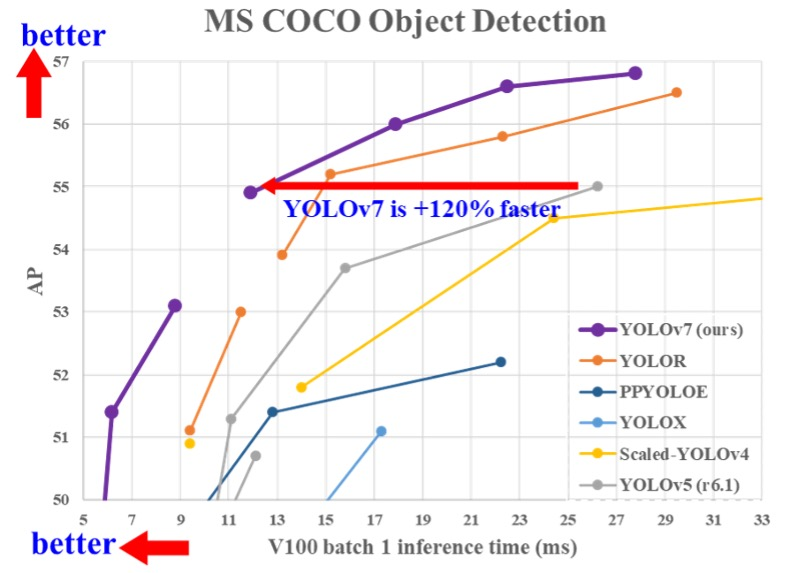
\includegraphics[width=0.7\textwidth]{yolov7_2.jpg}         %圖片檔案名稱
    \caption{YOLOv7與其它模型比較\cite{wang2023yolov7}}           %圖片檔案名稱
    \label{fig:yolov7_2}                                        %為圖片添加標籤
    %(如圖\ref{fig:yolov7_2} 所示)
\end{figure}

\begin{figure}[H]
    \centering
    \renewcommand{\figurename}{圖} %顯示圖1,不是figureat1
    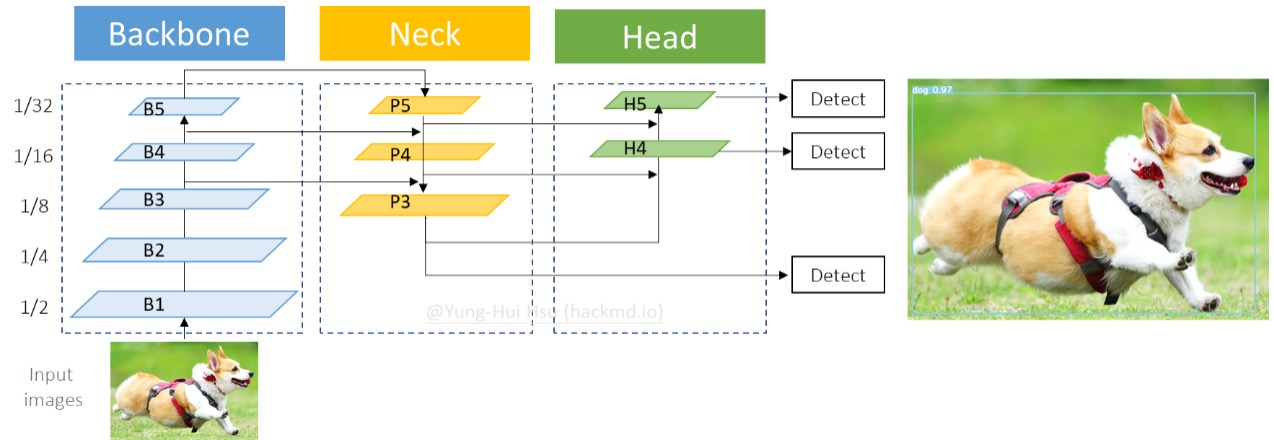
\includegraphics[width=0.7\textwidth]{yolov7_3.jpg}     %圖片檔案名稱
    \caption{YOLOv7架構圖\cite{hackmd}}    %圖片檔案名稱
    \label{fig:yolov7_3}    %為圖片添加標籤
    %(如圖\ref{fig:yolov7_3} 所示)
\end{figure}
%==============================內文==============================

\subsection{應用VBS-RTK之GPS定位}
%==============================內文==============================
\hspace{2em}在定位方面採用即時動態定位技術(Virtual Base Station Real-Time Kinematic, VBS-RTK)以獲得無人機精確位置,VBS-RTK是e-GNSS 即時動態定位系統之核心定位技術。
其係採用多個衛星定位基準站所組成的 GNSS 網絡來評估基準站涵蓋地區之定位誤差,再配合最鄰近的實體基準站觀測資料,產製一個虛擬的基準站做為RTK主站,所以移動站並不是接收某個實體基準站之實際觀測資料,而是經過誤差修正後的虛擬觀測數據。

\begin{figure}[H]
    \centering
    \renewcommand{\figurename}{圖}                              %顯示圖1,不是figureat1
    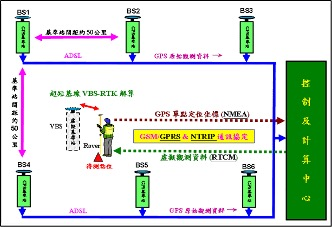
\includegraphics[width=0.7\textwidth]{vbsrtk.jpg}         %圖片檔案名稱
    \caption{VBS-RTK運作流程圖\cite{egnss_2020}}           %圖片檔案名稱
    \label{fig:vbsrtk}                                        %為圖片添加標籤
    %(如圖\ref{fig:yolov7_2} 所示)
\end{figure}
%==============================內文==============================

\subsection{影像處理與空間對位}
%==============================內文==============================
\hspace{2em}本計畫將利用鏡頭往斜下的角度拍攝而非垂直向下。以斜下角度拍攝的特點是相較於垂直向下拍攝可以擁有較大的視野範圍。
這部分需應用航空攝影測量原理\cite{zhao2013}的中共線方程式(Collinearity equation)求得地面點在像片上對應之坐標,共線方程式係基於透視中心投影之原則下根據物點、像點、以及攝影時的參數所建立,求得每一地面點在相片上對應之坐標。

\begin{figure}[H]
    \centering
    \renewcommand{\figurename}{圖}                              %顯示圖1,不是figureat1
    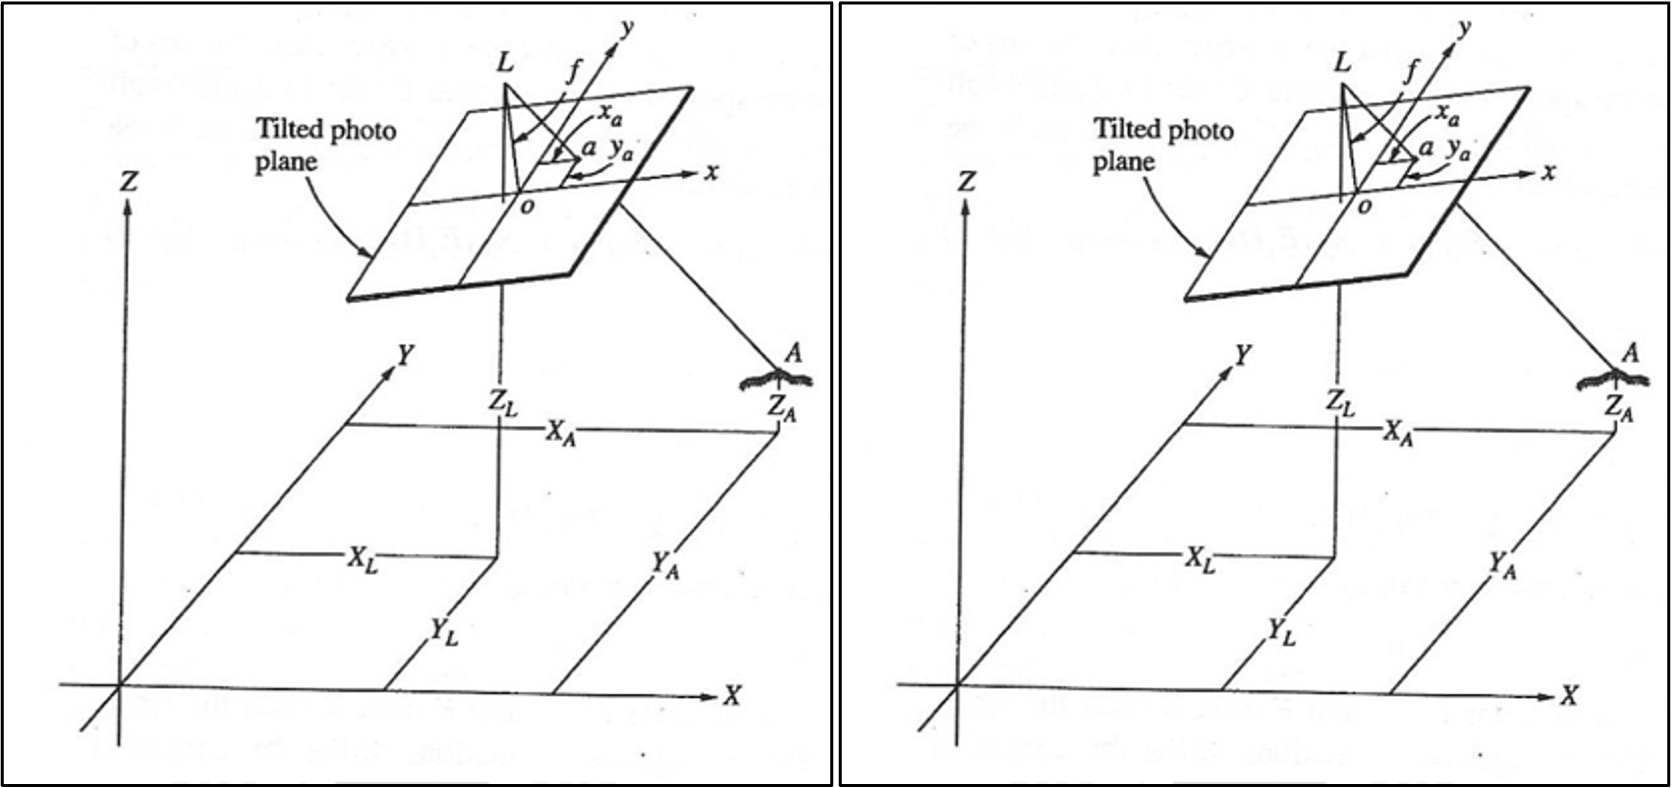
\includegraphics[width=0.7\textwidth]{ce.jpg}         %圖片檔案名稱
    \caption{共線式幾何示意圖\cite{tsao2018}}           %圖片檔案名稱
    \label{fig:ce}                                        %為圖片添加標籤
    %(如圖\ref{fig:yolov7_2} 所示)
\end{figure}
%==============================內文==============================

\section{\centering 研究方法及流程}
%==============================內文==============================
\hspace{2em}本計畫要設計的電腦應用程式,能夠標示出地圖中不可停車的區域,而無人機則透過事先建立的資料庫,
比對飛越指定區域所拍攝的影像,快速辨識違規車輛並記錄其車牌號碼,運作流程如\ref{fig:flow_chart}所示。
\begin{figure}[H]
    \centering
    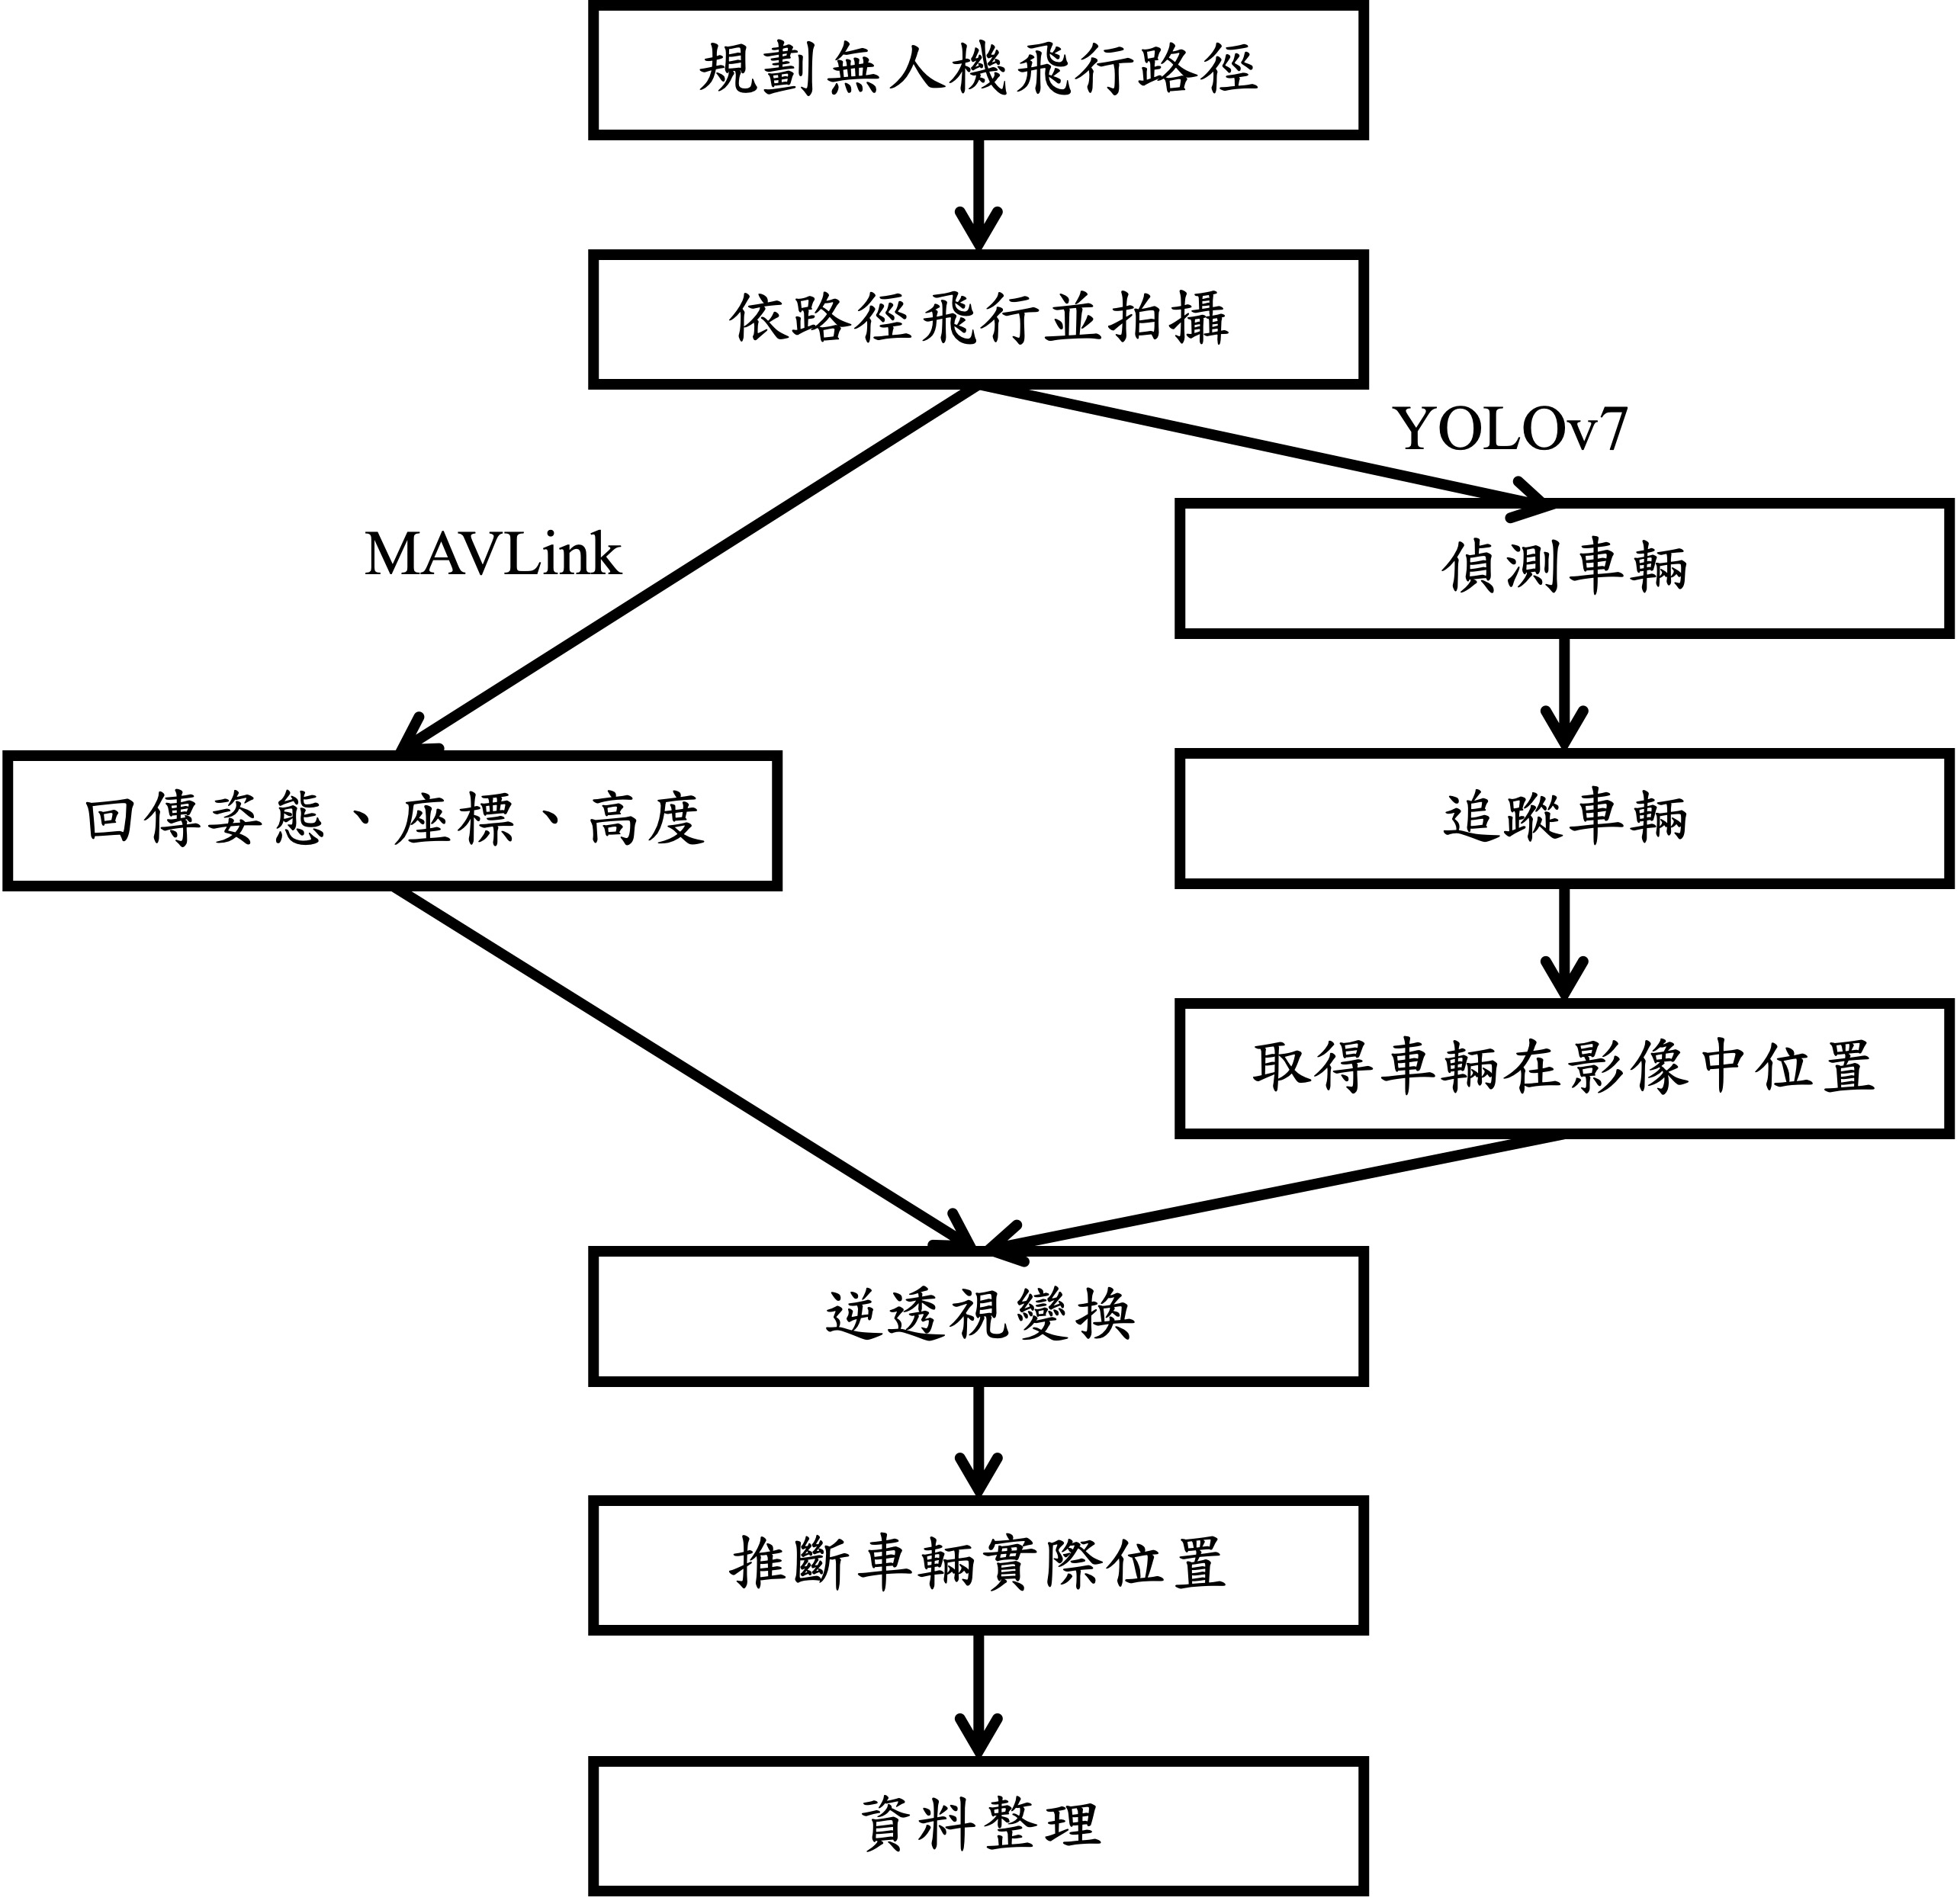
\includegraphics[width=0.7\textwidth]{flow_chart.jpg}     %圖片檔案名稱
    \caption{研究流程圖}    %圖片檔案名稱
    \label{fig:flow_chart}    %為圖片添加標籤
    %如\ref{fig:flow_chart}所示
\end{figure}
本研究中所使用的無人機,為委託臺灣希望創新股份有限公司(Taiwan Hope Innovation Corporation)所特別製作的無人機,實驗中使用的無人機為含有 Pixhawk4 Orange飛控板、樹梅派、GPS、HUAWEI 4G USB 網卡和 Logitech C922 Pro Stream單目攝像頭(具體規格詳見表\ref{tab:C922 Pro})的四軸飛行器。
錄製到的影像透過無人機上的樹梅派傳送到RTMP server \cite{chen2011}\cite{mark2018}。在由其他電腦從RTMP server取得影像並做辨識。為了使無人機飛行更順利,無人機上含有高性能的飛控板、精確的 GPS 定位系統,在兩者相互搭配下,使無人機有更穩定的飛行。

\begin{figure}[H]
    \centering
    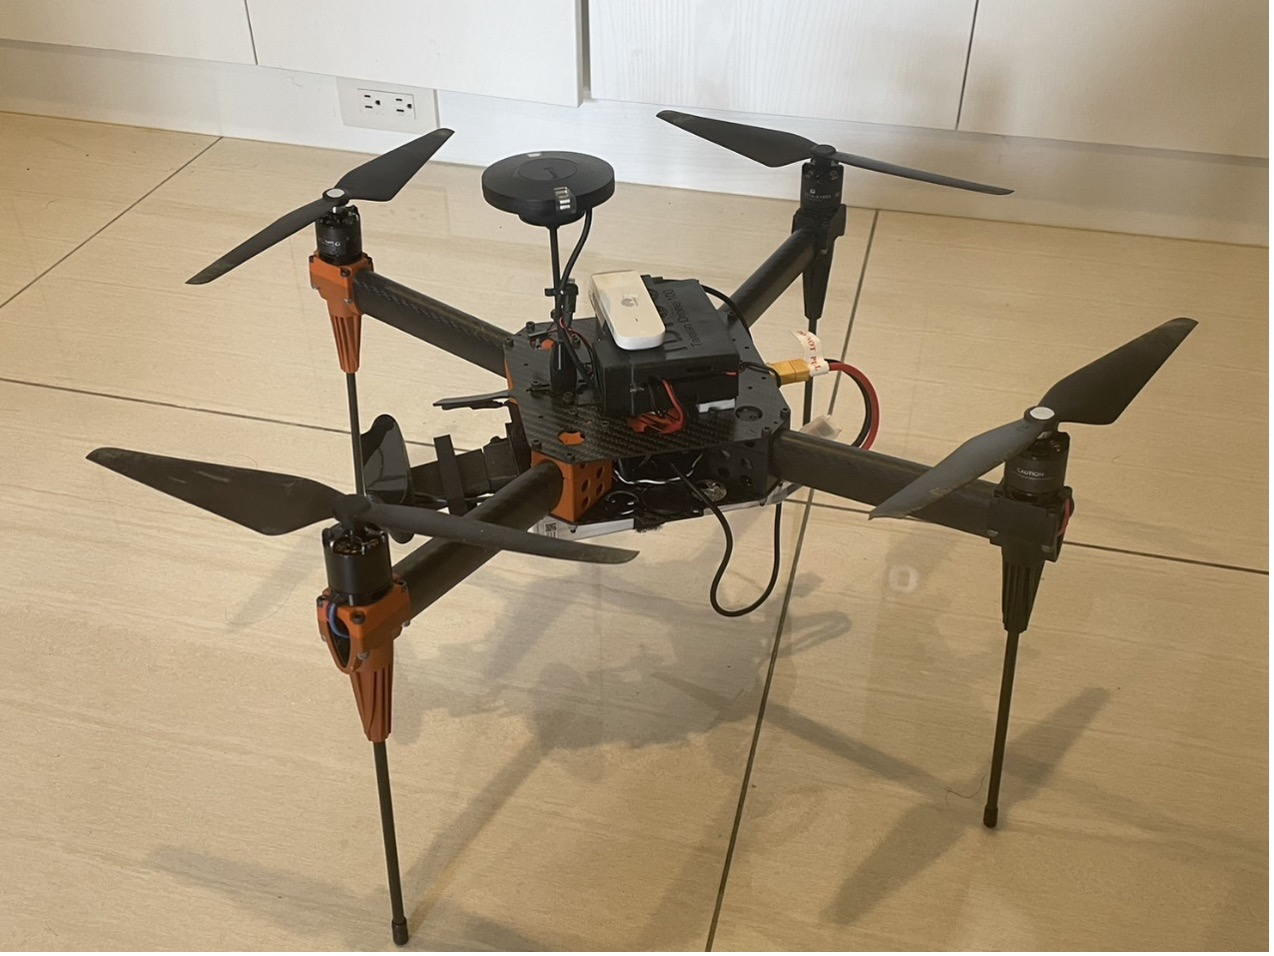
\includegraphics[width=0.7\textwidth]{UAVphoto.jpg}     %圖片檔案名稱
    \caption{本研究所使用之無人機}    %圖片檔案名稱
    \label{fig:UAVphoto}    %為圖片添加標籤
    %如\ref{fig:example1}所示
\end{figure}

\begin{figure}[H]
    \centering
    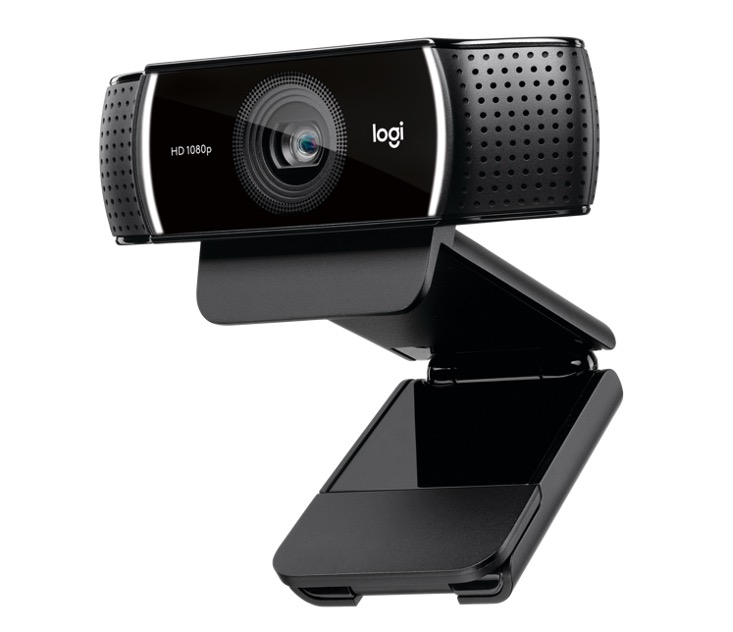
\includegraphics[width=0.7\textwidth]{c922.jpg}     %圖片檔案名稱
    \caption{本研究使用之單目攝像頭\cite{logitech}}    %圖片檔案名稱
    \label{fig:c922}    %為圖片添加標籤
    %如\ref{fig:c922}所示
\end{figure}

\begin{table}[H]
    \caption{C922 Pro Stream 規格}
    \vspace{12pt} % 增加空格
    \renewcommand{\arraystretch}{1.5} % 調整行距以垂直置中
    \centering
    \begin{tabular}{|c|c|}
        \hline
        項目   & 規格              \\ \hline
        解析度  & 1280$\times$720 (HD) \\ \hline
        幀率   & 30fps           \\ \hline
        水平視角 & 70.42$^\circ$         \\ \hline
        垂直視角 & 43.3$^\circ$           \\ \hline
    \end{tabular}
    \label{tab:C922 Pro}
    %(具體規格詳見表\ref{tab:C922 Pro})
\end{table}

無人機控制方面透過4G網卡及VPN以遠端控制樹莓派,並且在樹莓派中我們透過MAVProxy(MAVLink Proxy)\cite{mavproxy_2023}指令將飛控板透過UDP方式連線至電腦端的Mission Planner\cite{pixhawk_2023},
Mission Planner 提供了一個實時的飛行監控界面(如圖\ref{fig:missionplanner}所示),可編輯飛行計劃,並記錄飛行數據。
\begin{figure}[H]
    \centering
    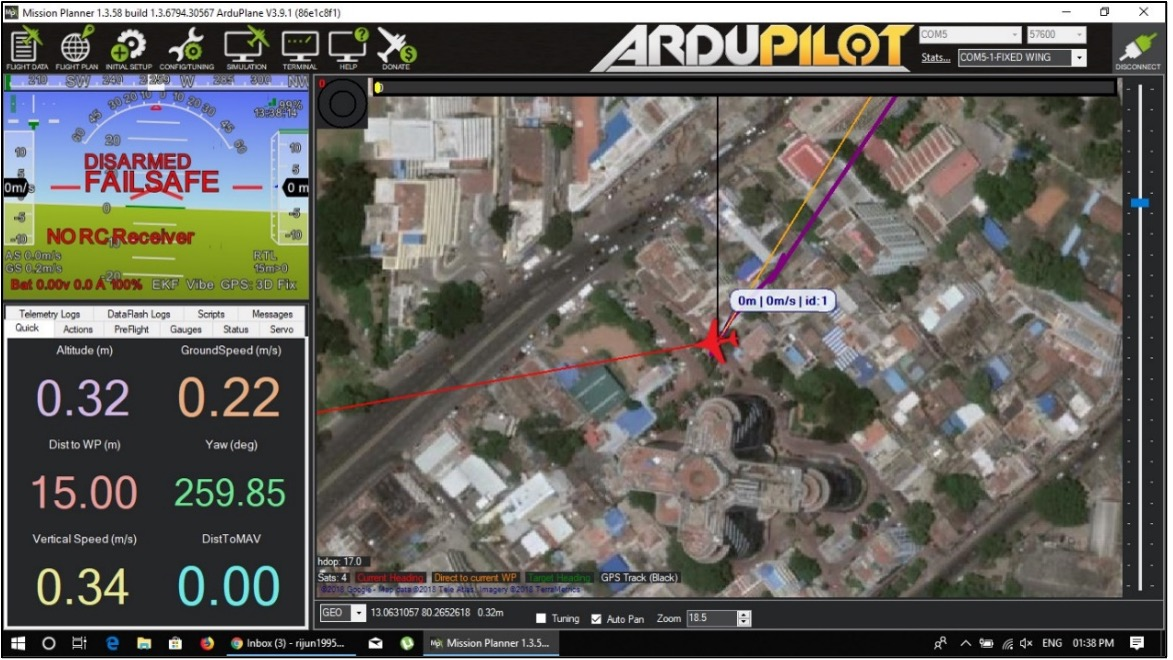
\includegraphics[width=0.7\textwidth]{missionplanner.jpg}     %圖片檔案名稱
    \caption{Mission Planner實際畫面\cite{pixhawk_2023}}    %圖片檔案名稱
    \label{fig:missionplanner}    %為圖片添加標籤
    %(如圖\ref{fig:missionplanner}所示)
\end{figure}
本實驗透過 4G 網路 連接無人機進行控制,並在電腦端使用 ROS 進行影像擷取與處理。
此外,在影像處理的同時,還需透過 Mission Planner 即時控制無人機並藉由 MAVLink 協議獲取相關資訊。
因此,筆記型電腦必須具備足夠的性能,以確保系統的穩定運行與即時回應。

本計畫中,主要使用 MSI GP76 Leopard 筆記型電腦(具體規格詳見表\ref{tab:MSI GP76 Leopard})。該機型以高效能為主打,搭載 Intel® Core™ i7-10870H 處理器與 NVIDIA® GeForce® RTX 3060 顯示卡,並採用 MSI 最新技術 Cooler Boost 5。其雙散熱模組設計、強力雙風扇與多組熱管,加上四向散熱氣流設計,能有效排除廢熱,確保處理器與顯示卡在高負載運行時維持最佳性能。
\begin{table}[H]
    \caption{MSI GP76 Leopard規格}
    \vspace{12pt} % 增加空格
    \renewcommand{\arraystretch}{1.5} % 調整行距以垂直置中
    \centering
    \begin{tabular}{|c|c|}
        \hline
        \textbf{元件} & \textbf{規格}                 \\ \hline
        中央處理器       & Intel\textregistered{} Core\texttrademark{} i7-10870H \\ \hline
        記憶體         & DDR4 16GB                   \\ \hline
        硬碟          & 1TB SSD                     \\ \hline
        顯卡          & NVIDIAl\textregistered{} GeForcel\textregistered{} RTX 3060   \\ \hline
        作業系統        & Ubuntu 18.04                \\ \hline
        電池          & 4-Cell 65 Battery (Whr)     \\ \hline
    \end{tabular}
    \label{tab:MSI GP76 Leopard}
    %(具體規格詳見表\ref{tab:MSI GP76 Leopard})
\end{table}
此外,本實驗也輔以 Apple MacBook M1 (具體規格詳見表\ref{tab:MacBook Air M1})進行部分運算與開發工作。MacBook M1 採用 Apple M1 晶片,內建 8 核心 CPU 及 7 核心 GPU,並配備 8GB 統一記憶體(Unified Memory),提供優異的效能與低功耗表現。在本研究中,MacBook M1 主要用於 ROS 1 相關開發、Python 影像處理、無人機數據分析與程式開發。
不過,由於 M1 晶片採用 ARM 架構,與傳統 x86 架構不同,在執行 ROS 及部分開發環境時,需透過 Docker 來確保軟體相容性。
\begin{table}[H]
    \caption{MacBook Air M1規格}
    \vspace{12pt} % 增加空格
    \renewcommand{\arraystretch}{1.5} % 調整行距以垂直置中
    \centering
    \begin{tabular}{|c|c|}
        \hline
        \textbf{元件} & \textbf{規格}            \\ \hline
        處理器         & Apple M1 (8 核心 CPU)    \\ \hline
        記憶體         & 8GB Unified Memory     \\ \hline
        硬碟          & 256GB SSD              \\ \hline
        顯示卡         & Apple M1 內建 GPU (7 核心) \\ \hline
        作業系統        & macOS Sequoia          \\ \hline
        電池          & 49.9Wh                 \\ \hline
    \end{tabular}
    \label{tab:MacBook Air M1}
    %(具體規格詳見表\ref{tab:MacBook Air M1})
\end{table}
綜合而言,MSI GP76 Leopard 主要負責高負載的影像處理與無人機控制,而 MacBook M1 則用於負責高負載的影像處理、程式開發與數據分析,兩者搭配可有效提升本實驗的運算效率與工作流程。
%==============================內文==============================

\subsection{飛行路徑規劃}
%==============================內文==============================
\hspace{2em}









%==============================內文==============================


\subsection{違規車輛偵測}
%==============================內文==============================
\hspace{2em}在車輛偵測方面,透過物件辨識技術YOLO(You Only Look Once),能夠高效、精確地辨識影像中的車輛。
YOLO是一種基於深度學習的物件偵測模型,能夠在單一的前向傳播過程中,同時進行分類與定位,從而達到快速處理的效果。
結合深度學習技術,YOLO能夠對車輛進行實時的辨識與定位,並在影像中標註出車輛的具體位置。
這不僅提高了車輛偵測的準確性,也能在多種複雜環境下有效運行,無論是白天、夜間,還是不同的天氣條件下。
藉由這些辨識出的資訊,系統可以進一步進行車輛是否違規的判斷。
\begin{figure}[H]
    \centering
    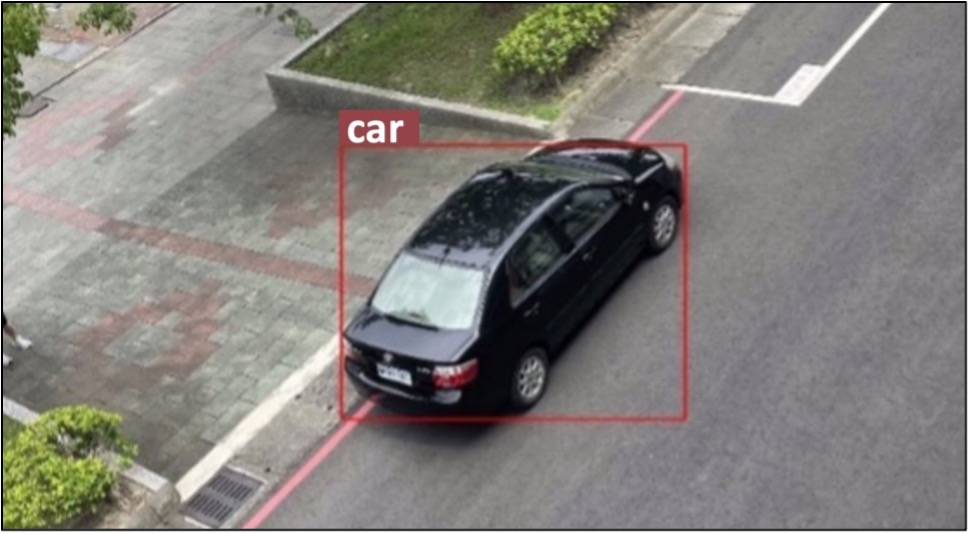
\includegraphics[width=0.7\textwidth]{yolov7car.jpg}     %圖片檔案名稱
    \caption{YOLOv8違規車輛偵測示意圖}    %圖片檔案名稱
    \label{fig:yolov7car}    %為圖片添加標籤
    %(如圖\ref{fig:yolov7car}所示)
\end{figure}
%==============================內文==============================

\subsection{影像處理}
%==============================內文==============================
\hspace{2em}無人機的座標系統定義如圖\ref{fig:xyzppr}所示。$y$軸的正方向為北方$x$軸與$y$軸垂直且以東方為正。
航向角$\psi$是以$yz$平面為基準,沿著$z$軸順時針旋轉的角度,範圍從0$^\circ$到360$^\circ$。
俯仰角$\theta$是以$xy$平面為基準,沿著$x$軸逆時針旋轉為正的角度,範圍從90$^\circ$到-90$^\circ$。
滾轉角$\phi$是以$xy$平面為基準,繞著$y$軸順時針旋轉的角度,範圍從-90$^\circ$到90$^\circ$。
無人機上的攝像頭默認朝向座標系的正$y$軸方向,攝像頭傾斜角度為$\theta_{c}$,範圍從0$^\circ$到-90$^\circ$,攝像頭位置與無人機重心距離忽略不計。
\begin{figure}[H]
    \centering
    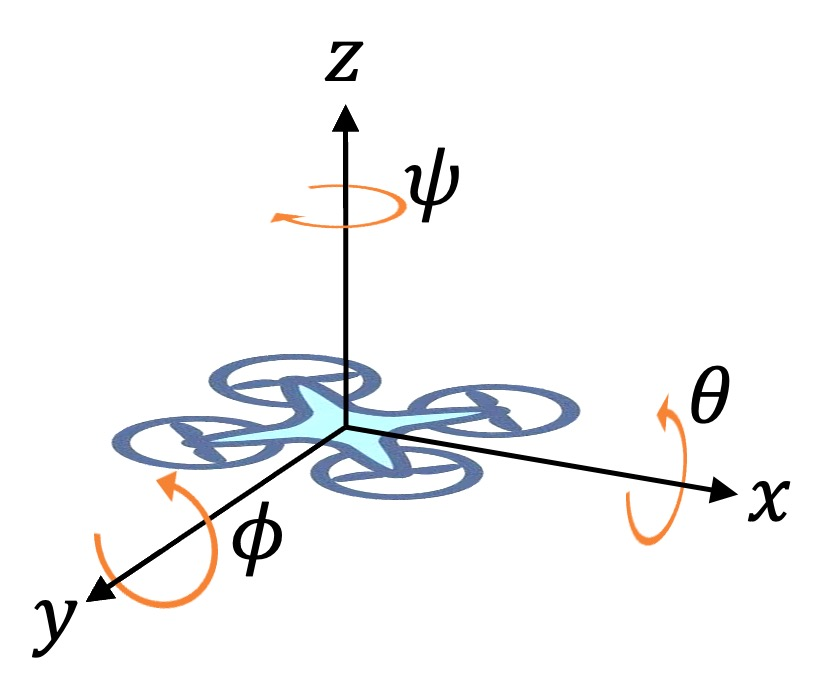
\includegraphics[width=0.7\textwidth]{xyzppr.jpg}     %圖片檔案名稱
    \caption{無人機座標系統定義}    %圖片檔案名稱
    \label{fig:xyzppr}    %為圖片添加標籤
    %(如圖\ref{fig:xyzppr}所示)
\end{figure}

本計畫將利用鏡頭往斜下的角度拍攝而非垂直向下,首先測試單純考慮無人機相機傾斜之投影,根據航空攝影測量原理\cite{zhao2013},可推導出以下公式。
$P_{r}(u_{r},v_{r})$照片上的一個點,$P_{v}(u_{v},v_{v})$為其在正射投影上的對應點(如圖\ref{fig:ipm} 所示)。以$A$表示為相片中心在鳥瞰圖上的對應點,並定為鳥瞰圖座標系的原點。$f$為焦距,原照片與正射投影的對應關係可由以下算式求得:
\begin{align}
    u_{v}=f\times\sec(\theta_{c}-\arctan\frac{v_{r}}{f})\times\frac{u_{r}}{\sqrt{v^2_{r}+f^2}} 
    \label{eq:uv}
    \\
    \label{eq:vv}        
    v_{v}=f\times(\tan\theta_{c}-\tan(\theta_{c}-\arctan\frac{v_{r}}{f}))              
\end{align}
\begin{figure}[H]
    \centering
    \renewcommand{\figurename}{圖}                              %顯示圖1,不是figureat1
    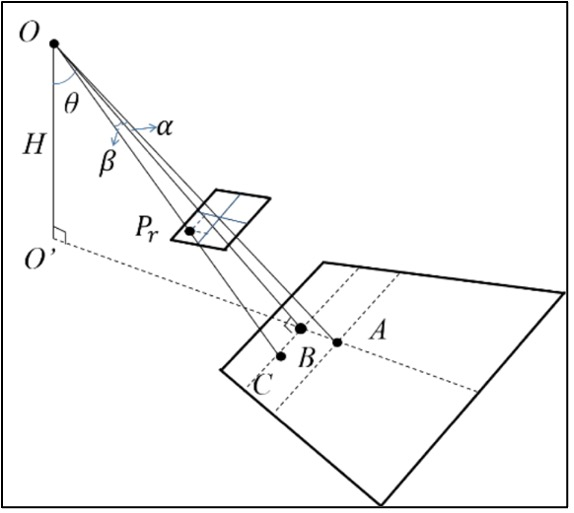
\includegraphics[width=0.7\textwidth]{ipm.jpg}         %圖片檔案名稱
    \caption{非垂直投影示意圖\cite{tsao2018}}           %圖片檔案名稱
    \label{fig:ipm}                                        %為圖片添加標籤
    %(如圖\ref{fig:ipm} 所示)
\end{figure}

本計畫將利用鏡頭往斜下的角度拍攝而非垂直向下,且飛行時會產生翻滾角 (Roll)、俯仰角(Pitch),以上因素皆會影響成像。
因此本研究採用逆透視變換(Inverse Perspective Mapping,IPM)\cite{lin_2001}\cite{bertozz1998stereo}\cite{mallot1991inverse}技術處理無人機拍攝的影像,以將像素座標轉換為地面座標,最後轉換成GPS座標。

首先將影像像素座標系$(u,v)$轉換為圖像座標系$(x,y)$。
加入相機的水平視角$HFOV$與相機的垂直視角$VFOV$、相機俯仰角$\theta_{c}$,無人機姿態則藉由 mavlink 從 mission planner 獲取俯仰角$\theta_{q}$、滾轉角$\phi_{q}$、航向角$\psi_{q}$,將圖像座標轉換為相機座標$(x_{c},y_{c},z_{c})$。
接著將相機座標系轉換為無人機標系$(x_w,y_w,z_w)$,以取得拍攝影像中內容物與無人機之相對位置。流程圖如下:
\begin{figure}[H]
    \centering
    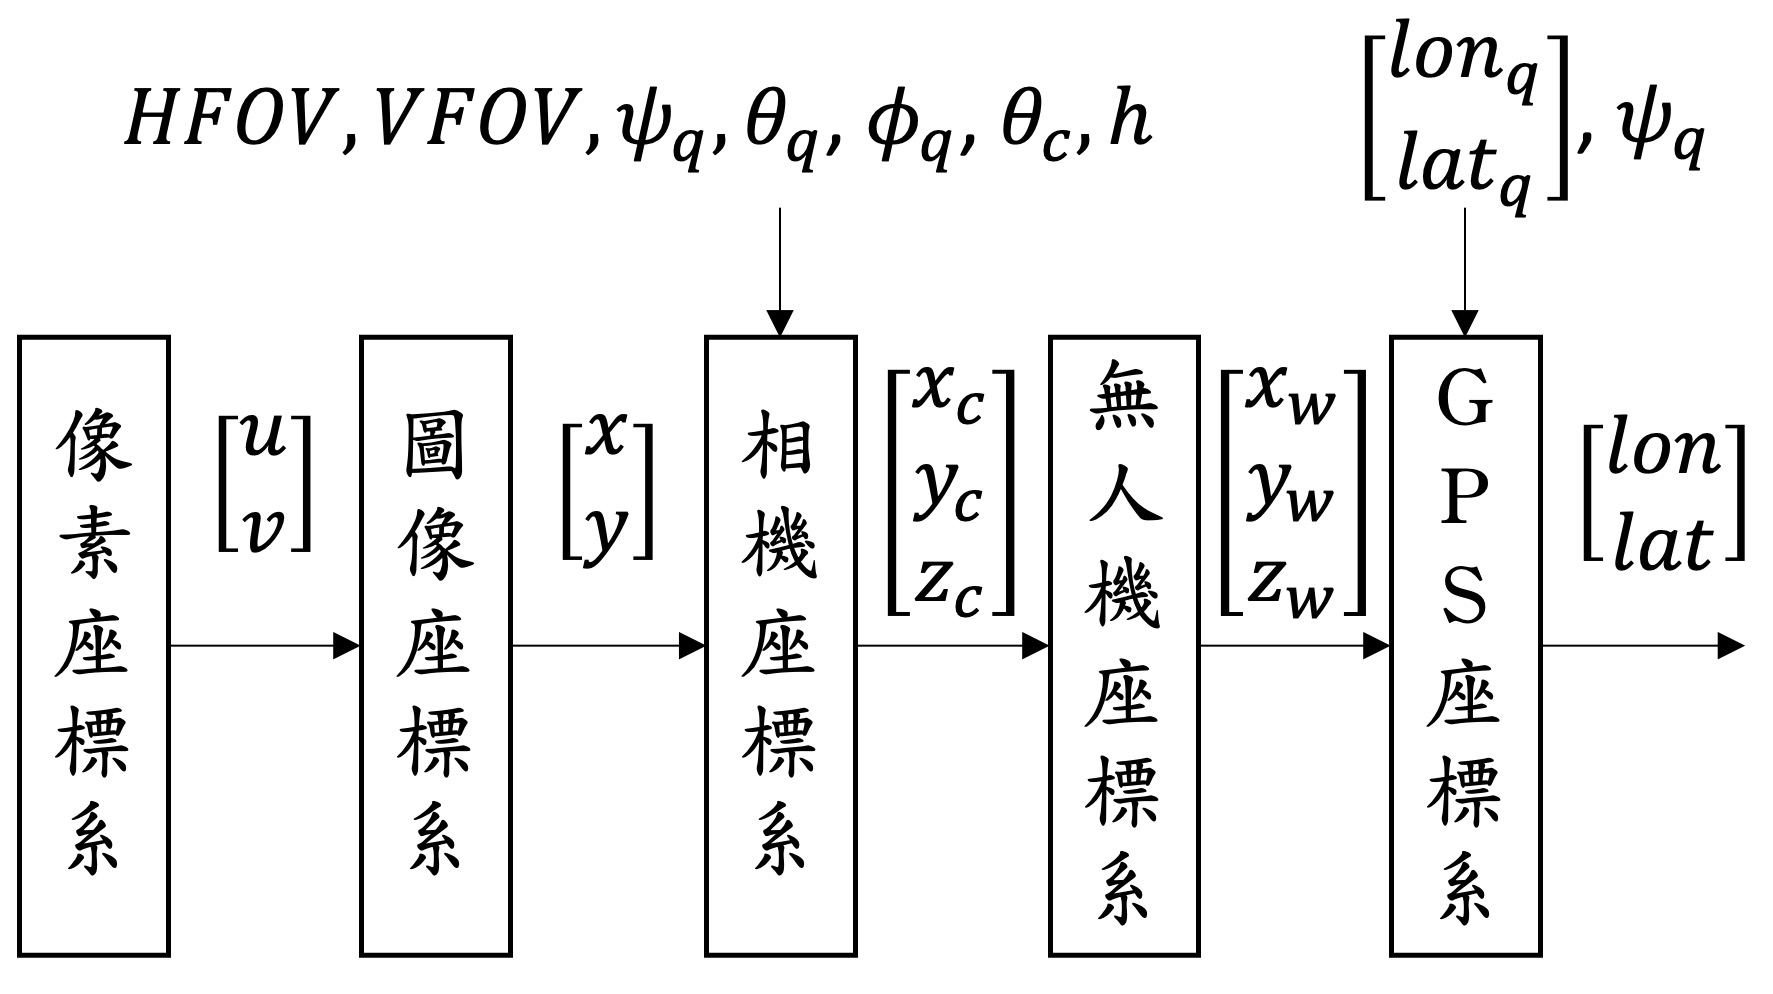
\includegraphics[width=0.7\textwidth]{pt.jpg}     %圖片檔案名稱
    \caption{座標轉換流程圖}    %圖片檔案名稱
    \label{fig:pt}    %為圖片添加標籤
    %(如圖\ref{fig:yolov7car}所示)
\end{figure}

將像素座標轉換為無人機相對於地平面的世界座標時,過程涉及相機的內參矩陣$K$、旋轉矩陣$R$以及無人機對地高度(相機高度)$h$。要算相機的內參矩陣首先需得出影像的水平焦距$f_{x}$、影像的垂直焦距$f_{y}$和影像的中心座標$(c_x,c_y)$。

影像的水平焦距$f_{x}$公式如式(\ref{eq:fx}),W為影像的寬度,HFOV為相機的水平視角。
影像的垂直焦距$f_{y}$公式如式(\ref{eq:fy}),H為影像的寬度,VFOV為相機的垂直視角。
\begin{align}
    f_{x}=\frac{W}{2\cdot\tan\left(\frac{HFOV}{2}\right)}
    \label{eq:fx}
    \\
    f_{y}=\frac{H}{2\cdot\tan\left(\frac{VFOV}{2}\right)}
    \label{eq:fy}
\end{align}

影像的中心座標$(c_x,c_y)$公式如式(\ref{eq:cx})、式(\ref{eq:cy}):
\begin{align}
    c_{x}=\frac{W}{2}
    \label{eq:cx}
    \\
    c_{y}=\frac{H}{2}
    \label{eq:cy}
\end{align}

式(\ref{eq:k})為相機內參矩陣K。
\begin{align}
    K &=
    \begin{bmatrix}
        f_{x}       & 0             & c_{x}     \\
        0           & f_{y}         & c_{y}     \\
        0           & 0             & 1
    \end{bmatrix} 
    \label{eq:k}
\end{align}

旋轉矩陣R用來表示相機相對於世界座標系的旋轉。無人機共有三個旋轉角度:俯仰角$\theta_{q}$、滾轉角$\phi_{q}$、航向角$\psi_{q}$。
航向角旋轉矩陣$R_{yaw}$、俯仰角旋轉矩陣$R_{pitch}$、滾轉角旋轉矩陣$R_{roll}$的公式分別是式(\ref{eq:ryaw})、式(\ref{eq:rpitch})、式(\ref{eq:rroll})。
\begin{align}
    R_{yaw} &=
    \begin{bmatrix}
        \cos\psi_{q}   & -\sin\psi_{q}  & 0 \\
        \sin\psi_{q}   & \cos\psi_{q}   & 0 \\
        0              & 0              & 1
    \end{bmatrix} 
    \label{eq:ryaw}
    \\
    R_{pitch} &=
    \begin{bmatrix}
        1   & 0  & 0 \\
        0   & \cos(\theta_{q}+\theta_{c})   & -\sin(\theta_{q}+\theta_{c}) \\
        0   & \sin(\theta_{q}+\theta_{c})   & \cos(\theta_{q}+\theta_{c})
    \end{bmatrix} 
    \label{eq:rpitch}
    \\
    R_{roll} &=
    \begin{bmatrix}
        \cos\phi_{q}    & 0     & \sin\phi_{q}  \\
        0               & 1     & 0             \\
        -\sin\phi_{q}   & 0     & \cos\phi_{q}
    \end{bmatrix} 
    \label{eq:rroll}
\end{align}

其組合的旋轉矩陣$R$如式(\ref{eq:R1})、式(\ref{eq:R2}):
\begin{align}
    R=R_{yaw}\cdot R_{pitch} \cdot R_{roll}
    \label{eq:R1}
\end{align}
\begin{align}
    R=
    \begin{bmatrix}
        \cos\psi_{q}   & -\sin\psi_{q}  & 0 \\
        \sin\psi_{q}   & \cos\psi_{q}   & 0 \\
        0              & 0              & 1
    \end{bmatrix} 
    \cdot
    \begin{bmatrix}
        1   & 0  & 0 \\
        0   & \cos(\theta_{q}+\theta_{c})   & -\sin(\theta_{q}+\theta_{c}) \\
        0   & \sin(\theta_{q}+\theta_{c})   & \cos(\theta_{q}+\theta_{c})
    \end{bmatrix} 
    \cdot
    \begin{bmatrix}
        \cos\phi_{q}    & 0     & \sin\phi_{q}  \\
        0               & 1     & 0             \\
        -\sin\phi_{q}   & 0     & \cos\phi_{q}
    \end{bmatrix} 
    \label{eq:R2}
\end{align}

將像素座標系$(x,y)$轉換為圖像座標系的公式如式(\ref{eq:xy1}):
\begin{align}
    \begin{bmatrix}
        x       \\
        y    \\
        1        
    \end{bmatrix} 
     &=K^{-1}\cdot
     \begin{bmatrix}
        u       \\
        v       \\
        1        
    \end{bmatrix} 
    \label{eq:xy1}
\end{align}

將圖像座標系轉換為相機座標系的公式如式(\ref{eq:xcyczc}):
\begin{align}
    \begin{bmatrix}
        x_{c}   \\
        y_{c}   \\
        z_{c}        
    \end{bmatrix} 
     &=R\cdot
     \begin{bmatrix}
        x       \\
        y       \\
        1        
    \end{bmatrix} 
    \label{eq:xcyczc}
\end{align}

將相機座標系轉換為世界座標系$(x_{w},y_{w},z_{w})$的公式見式式(\ref{eq:xw})、式式(\ref{eq:yw}),此公式即可獲的以無人機(相機)與偵測到的車輛之相對位置。
\begin{align}
    x_{w}=\frac{x_{c}}{z_{c}}
    \label{eq:xw}\\
    y_{w}=\frac{y_{c}}{z_{c}}
    \label{eq:yw}
\end{align}

在最後的整合階段,無人機的 GPS 位置作為已知參考點,結合車輛與無人機之間的相對位置,透過 Pyproj 函式庫\cite{pyproj}將這些相對位置轉換為標準的 GPS 坐標。
Pyproj 是基於 PROJ 庫的強大 Python 座標轉換與地理投影工具,專為地理資訊系統(GIS)設計。它提供靈活且精確的座標系統轉換功能,能夠在全球與區域性坐標系統之間進行準確變換,廣泛應用於地圖服務、導航、遙測影像分析等領域。
%==============================內文==============================

\subsection{空間對位}
%==============================內文==============================
\hspace{2em}透過獲取無人機的絕對位置以及相關的飛行參數,可以應用透視變換技術,將無人機拍攝的影像中的像素座標轉換為相對應的GPS座標。
這一過程不僅能夠將影像中的物體位置準確地映射到真實的地理座標系統中,還可以達成對影像位置的精確校正,實現空間對位。
在此基礎上,空間對位的技術將被應用於QGIS(Quantum GIS)\cite{QGIS_software},這是一款開源的桌面地理信息系統應用程序,廣泛應用於地理數據的分析與處理。

QGIS支持各種地理信息數據格式,並提供豐富的工具與功能,幫助用戶進行數據的導入、匯出及分析。在這項研究中,我將使用QGIS進行空間對位,驗證無人機所拍攝影像中車輛位置的準確性,並與實際地面的位置進行比對。
透過無人機的拍攝影像,可以提取影像中的車輛位置,並將其與已知的GPS座標進行對比。
\begin{figure}[H]
    \centering
    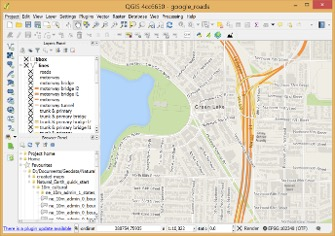
\includegraphics[width=0.7\textwidth]{qgis.jpg}     %圖片檔案名稱
    \caption{QGIS操作畫面\cite{qgis_2020}}    %圖片檔案名稱
    \label{fig:qgis}    %為圖片添加標籤
    %如\ref{fig:qgis}所示
\end{figure}
利用透視變換,將影像中的像素座標轉換成地理座標,並使用QGIS來執行這些座標的空間對位,將影像中的車輛位置對應到地面實際的位置。
接著,將這些透視變換計算得出的GPS座標與現場實際測量得到的GPS座標進行比對,以檢視兩者之間的誤差,從而評估該方法在實際應用中的精度與可靠性。
此方法不僅能夠驗證無人機拍攝影像的地理位置準確性,還能夠提供精確的車輛位置追蹤。
%==============================內文==============================


\section{\centering 研究結果}
%==============================內文==============================
\hspace{2em}研究結果主要分成幾部分

%==============================內文==============================

\subsection{飛行路徑規劃}
%==============================內文==============================
\hspace{2em}









%==============================內文==============================

\subsection{IMU資料獲取}
%==============================內文==============================
\hspace{2em}
\begin{figure}[H]
    \centering
    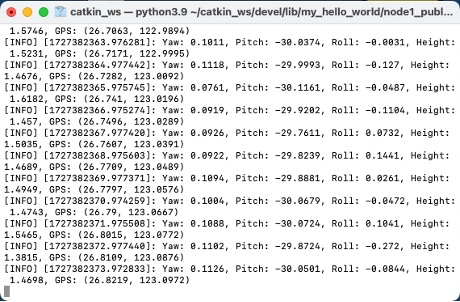
\includegraphics[width=0.7\textwidth]{mavlink.jpg}     %圖片檔案名稱
    \caption{mavlink}    %圖片檔案名稱
    \label{fig:mavlink}    %為圖片添加標籤
    %(如圖\ref{fig:mavlink}所示)
\end{figure}
%==============================內文==============================

\subsection{車輛偵測}
%==============================內文==============================
\hspace{2em}
\begin{figure}[H]
    \centering
    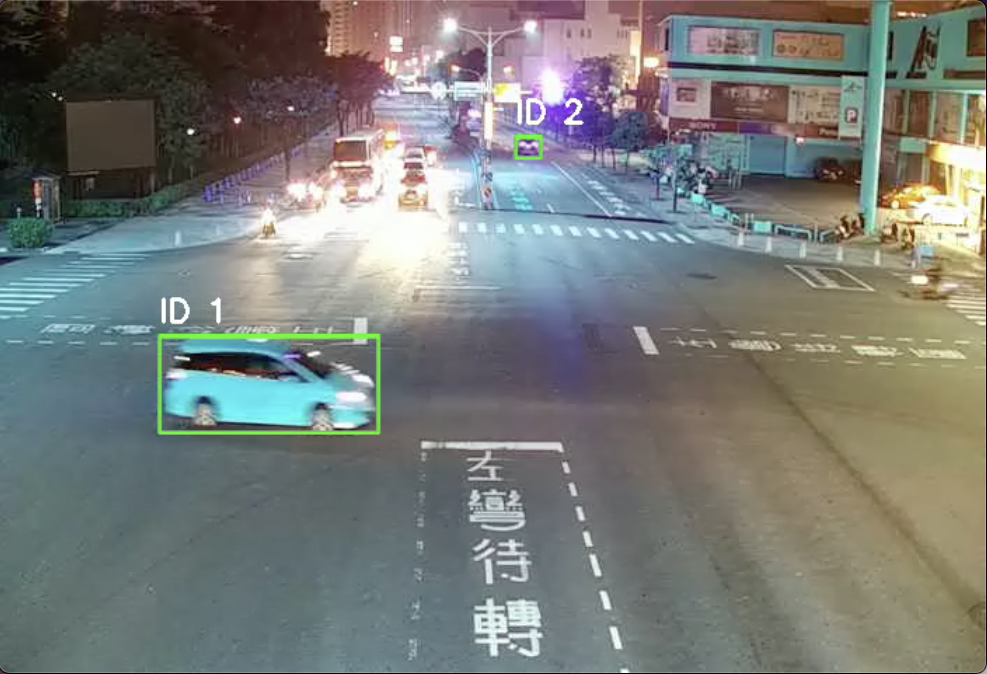
\includegraphics[width=0.7\textwidth]{yoloreal2.png}     %圖片檔案名稱
    \caption{Yolov7車輛偵測與追蹤}    %圖片檔案名稱
    \label{fig:yoloreal}    %為圖片添加標籤
    %(如圖\ref{fig:yoloreal2}所示)
\end{figure}
\begin{figure}[H]
    \centering
    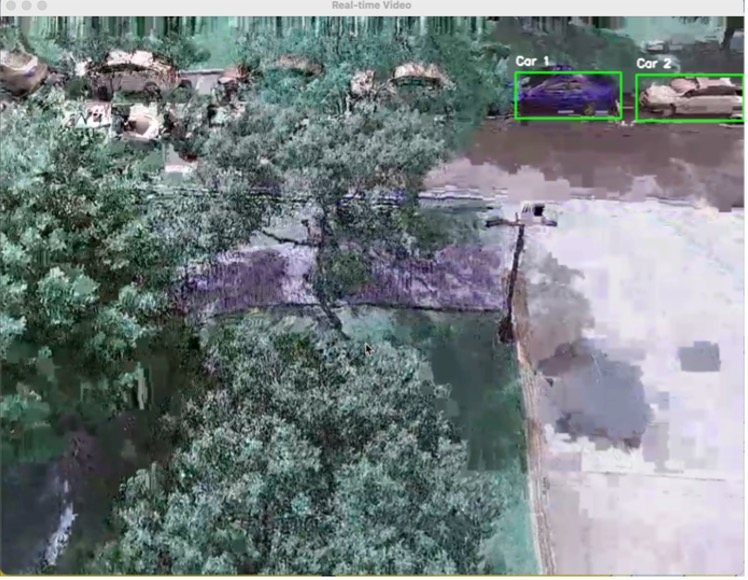
\includegraphics[width=0.7\textwidth]{yoloreal1.jpg}     %圖片檔案名稱
    \caption{Yolov7車輛偵測與追蹤-無人機實拍}    %圖片檔案名稱
    \label{fig:yoloreal1}    %為圖片添加標籤
    %(如圖\ref{fig:yoloreal1}所示)
\end{figure}
%==============================內文==============================

\subsection{影像處理}
%==============================內文==============================
\hspace{2em}

%==============================內文==============================

\subsection{逆透視變換}
%==============================內文==============================
\hspace{2em}
\begin{figure}[H]
    \centering
    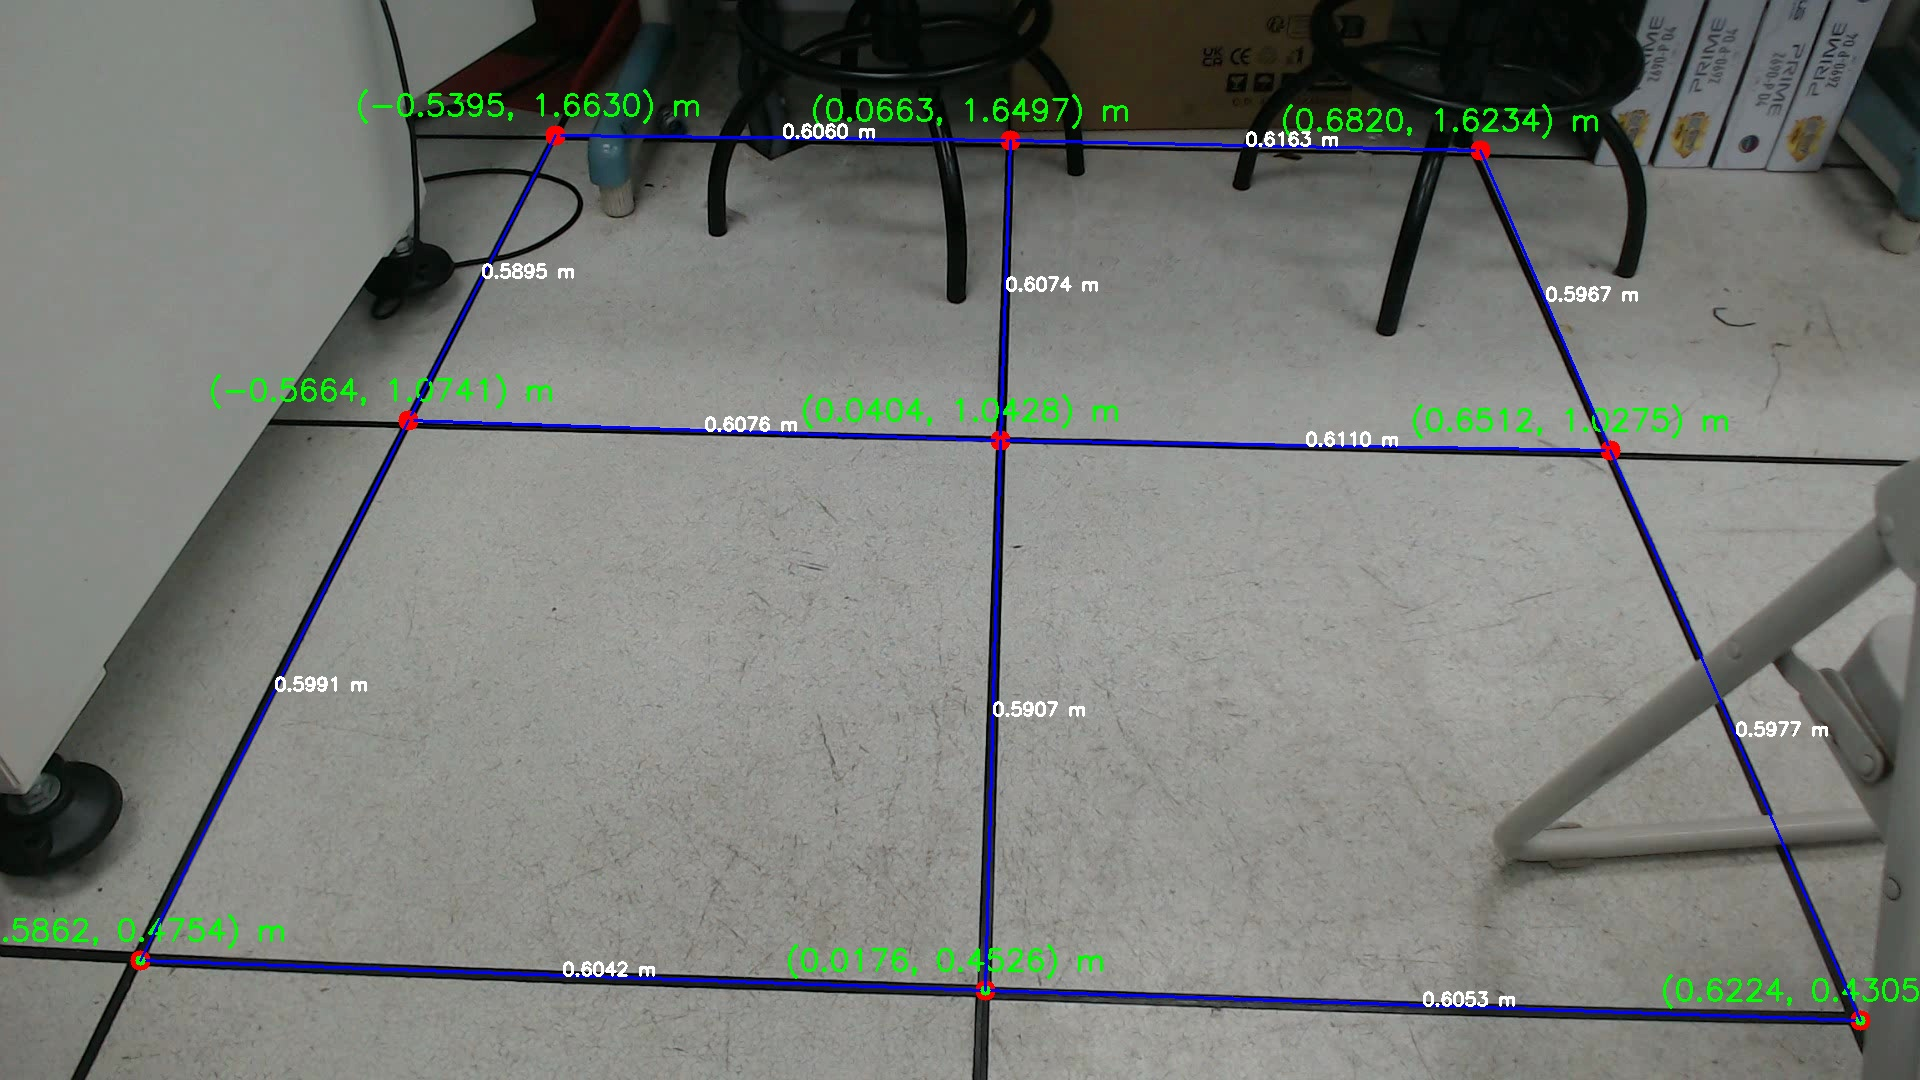
\includegraphics[width=0.7\textwidth]{frame_with_points_real.jpg}     %圖片檔案名稱
    \caption{地板測試}    %圖片檔案名稱
    \label{fig:frame_with_points_real}    %為圖片添加標籤
    %(如圖\ref{fig:frame_with_points_real}所示)
\end{figure}
%==============================內文==============================

\subsection{空間對位}
%==============================內文==============================
\hspace{2em}
\begin{figure}[H]
    \centering
    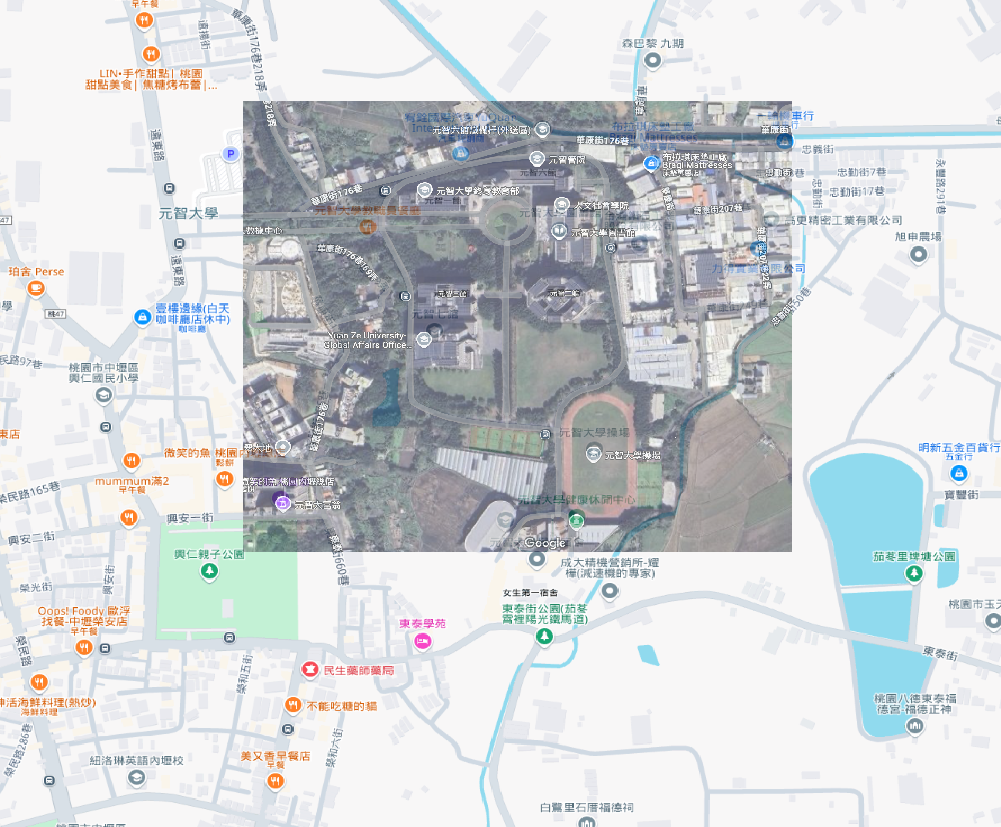
\includegraphics[width=0.7\textwidth]{1234567890.png}     %圖片檔案名稱
    \caption{空間對測試}    %圖片檔案名稱
    \label{fig:1234567890}    %為圖片添加標籤
    %(如圖\ref{fig:1234567890}所示)
\end{figure}
%==============================內文==============================

\section{\centering 結論} 
%==============================內文==============================
\hspace{2em}


%==============================內文==============================

\section{\centering 參考文獻}
\vspace{-3.5em}  % 減少與上方內容的間距
\renewcommand{\refname}{}  % 去除 "References" 標題
\printbibliography  % 列出參考文獻

\end{document}

%=============================================================================================================================
%=============================================================================================================================
%=============================================================================================================================


\begin{comment}
    %==============================圖片==============================
\begin{figure}[H]
    \centering
    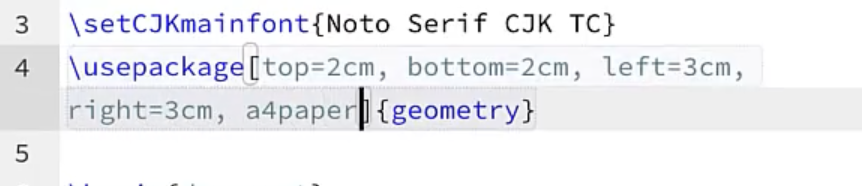
\includegraphics[width=0.7\textwidth]{截圖 2025-01-24 03.21.17.jpg}     %圖片檔案名稱
    \caption{這是圖片的標題}    %圖片檔案名稱
    \label{fig:example2}    %為圖片添加標籤
    %如\ref{fig:example1}所示
\end{figure}
    
    %==============================數學公式==============================
\begin{align}
    a &= b + c \label{eq:1}
    \\
    d &= e - f \label{eq:2}
    %式label{eq:2}
\end{align}
    
    %==============================表格==============================
\begin{table}[H]
    \caption{MSI GP76 Leopard規格}
    \vspace{12pt} % 增加空格
    \renewcommand{\arraystretch}{1.5} % 調整行距以垂直置中
    \centering
    \begin{tabular}{|c|c|}
        \hline
        \textbf{元件} & \textbf{規格}                 \\ \hline
        中央處理器       & Intel(R) Core(TM) i7-10870H \\ \hline
        記憶體         & DDR4 16GB                   \\ \hline
        硬碟          & 1TB SSD                     \\ \hline
        顯卡          & NVIDIA® GeForce® RTX 3060   \\ \hline
        作業系統        & Ubuntu 18.04                \\ \hline
        電池          & 4-Cell 65 Battery (Whr)     \\ \hline
    \end{tabular}
    \label{tab:MSI GP76 Leopard}
    %(具體規格詳見表\ref{tab:MSI GP76 Leopard})
\end{table}
    
    \end{comment}
        